\documentclass[a4paper,UKenglish]{article}
\usepackage[utf8]{inputenc}
\usepackage{fontenc,url}
\usepackage{babel,textcomp}
\usepackage[round]{natbib}
\usepackage{graphicx}
\usepackage{subcaption}
\graphicspath{ {images/} }
%\urlstyle{sf}

\title{Report1}
\author{Kasper Skjegggestad}
\begin{document}
\maketitle
\tableofcontents

\section{Introduction}

Digital elevation models (DEM), or digital terrain models (DTM) are widely used in research by scientists in governmental, university and private organizations. It is particularly useful for for geoscientific applications such as glaciers and rock-glaciers, geomorphology and georisk, hydrology, and land cover/ land use \citep{toutin08}. By analyzing DEMs you can, among other things, estimate were a landslide might originate, estimate precipitations zones or estimate the volume changes of a glacier. All researches based on DEMs will be dependent on the quality of the DEM. The quality of a DEM depends on the method of how it was collected and generated. DEM can be generated with inSAR, LiDAR, and with stereoscopy. The last method will be used to generate a DEM of Jotunheimen from ASTER in this study. The DEM will then be compared with DEMs generated from kartverket and silcAst over the same area. The same stereo image that was used to generate a DEM will be orthorectified by the new DEM, and compared to the image orthorectified kartverkets DEM.

\section{Goal}

The goal of this study is to generate a DTM from ASTER stereo images, orthorectify it, and assess accuracy of the DTM. The DTM and the ortophoto will be compared to DTM from Statens kartvert and DTM generated from silcAst. 

\section{Data}

Stereo images have been taken over Jotunheimen by ASTER on 12. Juli 2004. Additional DEM was provided by SilcAst and from Staten Kartverk. Theres DEM will be used to check the accuracy of the DEM that are to be generated from ASTER stereo images. The DEM from kartverket was also used to gather elevation for the GCPs. A map was optaint from statens kartverk in order to gather the coordinates for the GCPs.

\section{ASTER DEM production}

The DEM was generated with ASTER stereo image data Level 1B in Geomatica of PCI. The first object, after loading the image into the software, was to collect Global Control Points (GCPs). On the NADIR image, recognizable places in the map was found. The GCPs consisted mostly of lakes and rivers, since they was easy to find in both pictures. The elevation and coordinates for the points was gathered from a DEM and maps from kartverket. Kartverket had a tile map consisting of 9 tiles over the area of interest. Each tile was used to ensure GCPs over the entire area. The points was then transfered to the back-looking image. Most GCPs had to be adjusted to represent the same point. 30 points was found altogether, however, the position of two of the points was outside the bordars of the backlooking image. Therese points was therefore put to "check" in the this image, so not to affect the DEM. The residual of the remaining points then ranged from 0.20 to 5.69 in the two images. Tie-points was then collected. PCI geomatica did this automatically for me.

Next i created an epipolar image with 3N and 3B, now i can extract DEM. In the interface of 'Extract DEM automatically', I changed the terrain to mountainous from hilly, and gave the DEM a spacial resolution of 60x60m.

\section{Orthoprojection}

The 'Ortho Generation' step in PCI was done with both 3N and 3B and with my own DEM and Statens Kartverk DEM.

\section{Results}

\begin{figure}
	\begin{subfigure}{.5\textwidth}
		  \centering
		  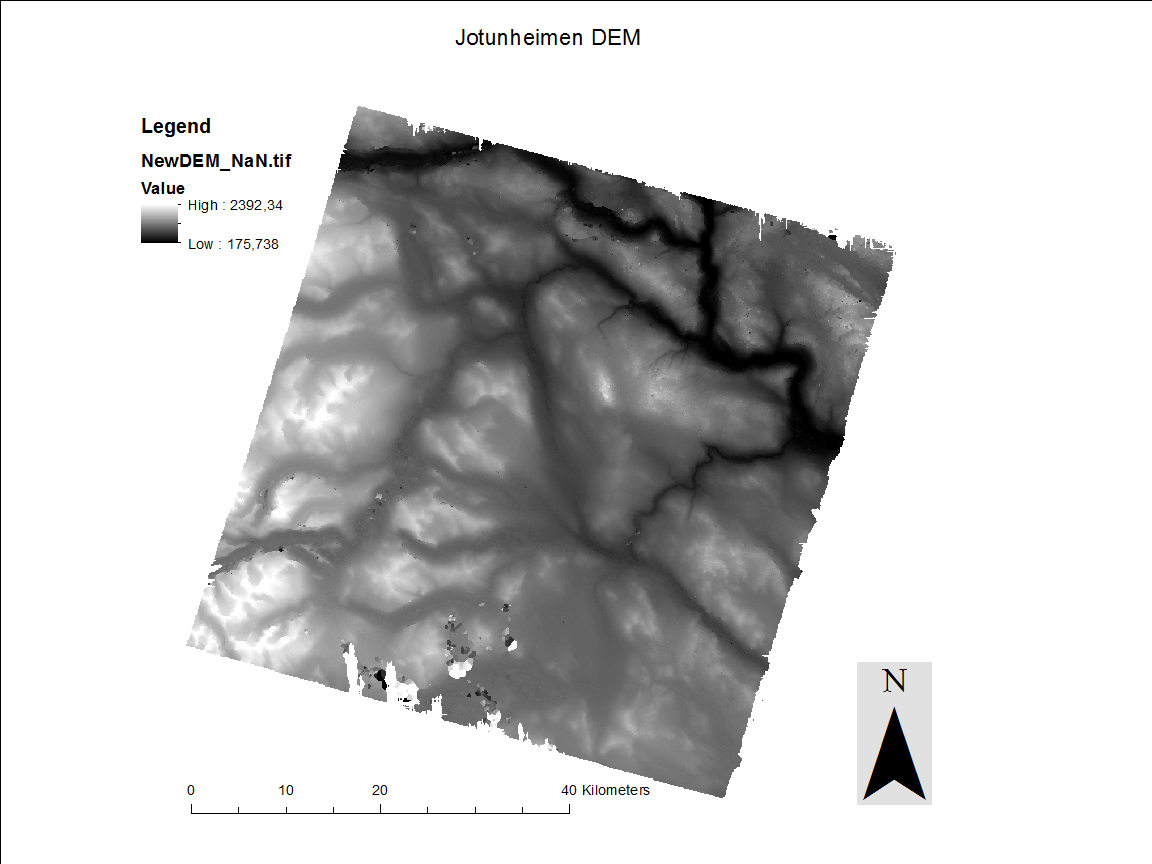
\includegraphics[height=5cm]{DEM_NAN}
		  \caption{DEM generated from aster stere images}
		  \label{dem}
	\end{subfigure}%
	\begin{subfigure}{.5\textwidth}
		  \centering
		  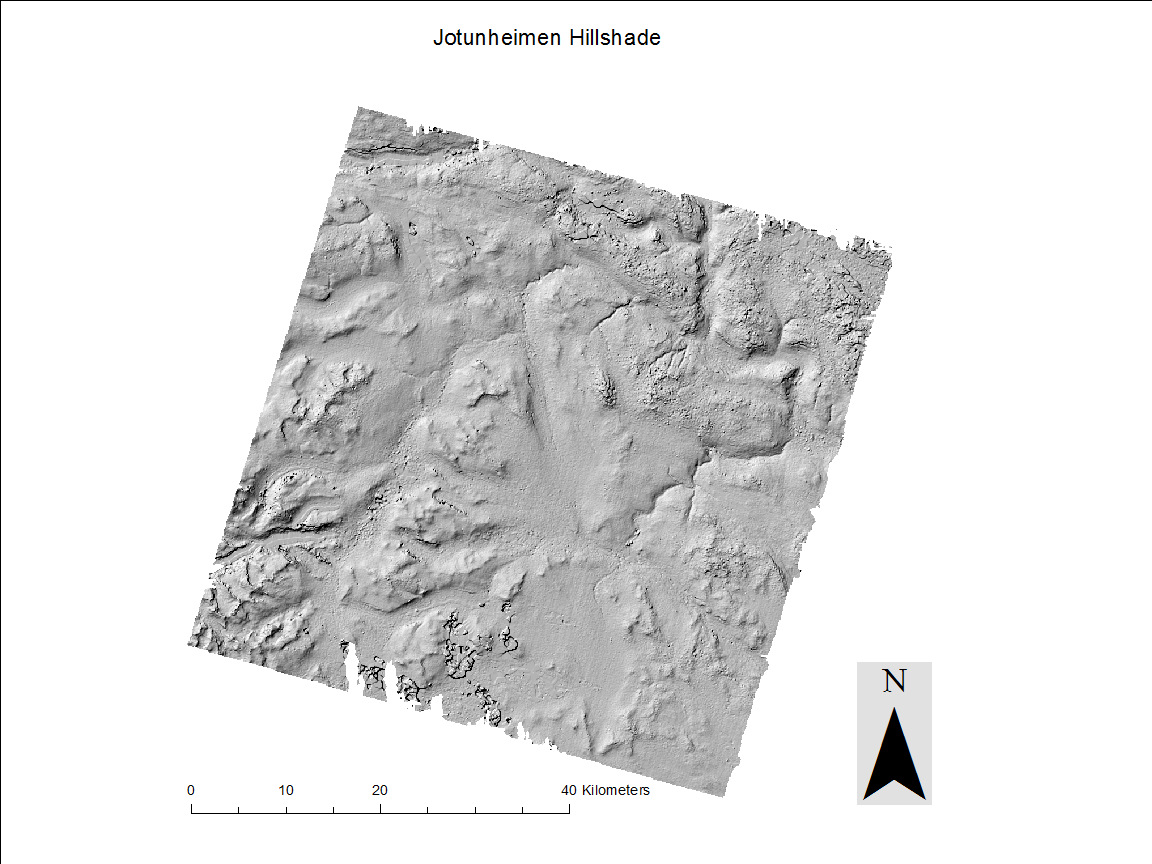
\includegraphics[height=5cm]{hillshade}
		  \caption{Hillshade generated from the new DEM}
		  \label{hillshade}
	\end{subfigure}
	\caption{Hillshade of the generated DEM and the generatet orthophotho}
	\label{hilldem}
\end{figure}

When the DEM and othophoto was generated, the files was uploaded to ArcMap for visualization and further operations. When the DEM was first visualized, only a gray image was shown. In areas where no data was found, the value -150 had been given. This made the range of the minimum and maximum values so big, that it become impossible to differentiate between any other values. To get around this, all values of -150 was set to NaN (Not a Number), and was thereby ignored.
In figure \ref{hilldem}, the DEM (\ref{dem}) and hillshade (\ref{hillshade}) are displayed. 

Viewing the newly generated DEM, some clear outliers are spottet. Some of these can easily be seen in a 3D representation of the DEM (figure \ref{3dimage}). On the left of figure \ref{3dimage}, there are some really high, steep "mountains" (a). This is clouds from the satellite image. The clouds are blocking the satellites view of the ground terrain, and we will therefor not get ground data in theres areas. A little left of the center in figure \ref{3dimage} (b), and to the right in the figure (c), tall black "mountains" can be spotted. Therese are located in lakes, and therefor there can not be any mountain or elevation difference here. This is errors that was obtained when generating the DEM. When adding contour lines over the orthophoto, some more errors are spotted. The small hills in the lakes are spotted, as well as massive gathering of contourlines around the clouds.

The difference between the newly generated DEM, kartverkets DEM and silcAst DEM are calculated in ArcMap using raster calculator. The result are then transfered to matlab to extract statistical information. The differences consist of rather large outliers, due to errors in the DEM. Outliers bigger then 3 standard derivatives ($3\sigma$) are removed. After the outliers have been removed, and the statistical operations are done, the differences between the DEMs are transfered back to ArcMap.

\begin{figure}
	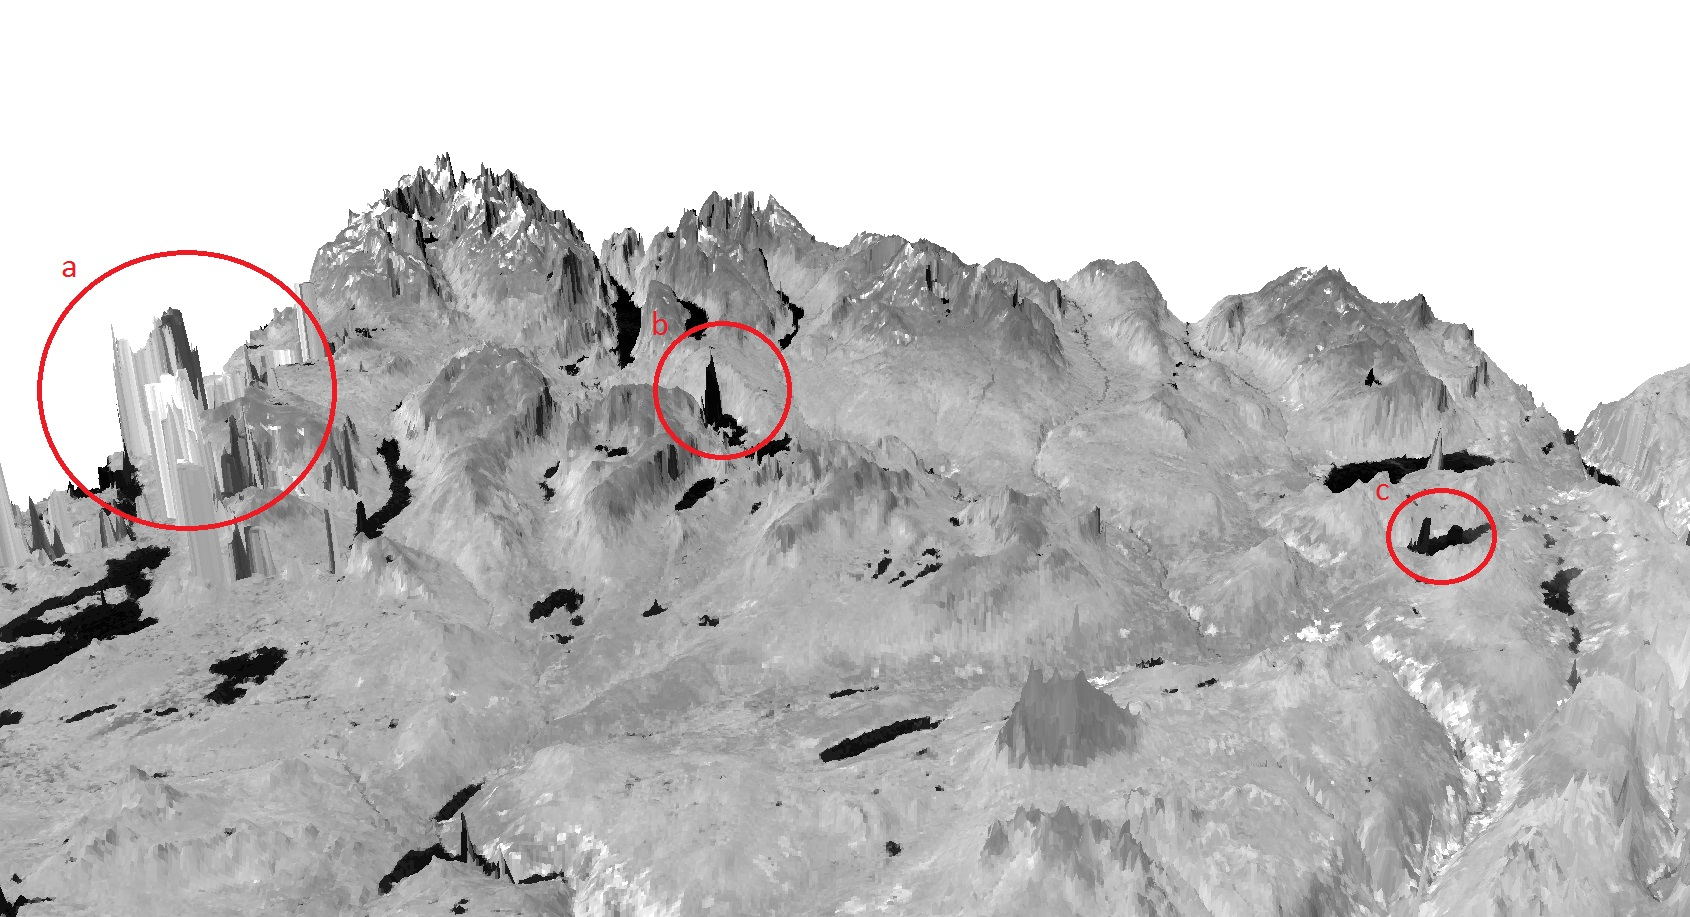
\includegraphics[height=6.7cm]{3dbilde3}
	\caption{3D representation of new DEM over ortopotho}
	\label{3dimage}
\end{figure}

\section{Analysis}

When visualizing the difference between the newly generated ASTER DEM, a DEM generated of silcast and karverkets DEM, it is reviled that the new DEM has larger errors in the south east and north west border and in the center parallel to theres borders (figure \ref{diffs}). In the borders figure \ref{diffs} shows a lots of green, witch mean the difference is negative. In the center, parallel to theres borders, the figure show a lots of red, symboling positive difference. This systematic error is not present when we look at the different between silcast and karverket, indicating that this error in the newly generated DEM only. It appears that the new DEMs south east and noth west borders have been raised, while the center parallel to therse borders have been lowerd, making the new DEM convex.

Parallel to the convection, some stripes are visible in the images of the new DEM differances. Therese stripes are not visible in the difference image of kartverkets DEM and silcast DEM. Therese lines might have something to do withe the fact thet the level 1B imgae was used, as this image a the raw image. Level 1B have been corrected corrected for the systematic distortions due to the sensor, the platform and the Earth rotating and curvature \citep{toutin01}. However, further investigation is recurred to know whether or not the stripes is a result of the corrections made on 1B.

\begin{figure}
	\begin{subfigure}{.5\textwidth}
		  \centering
		  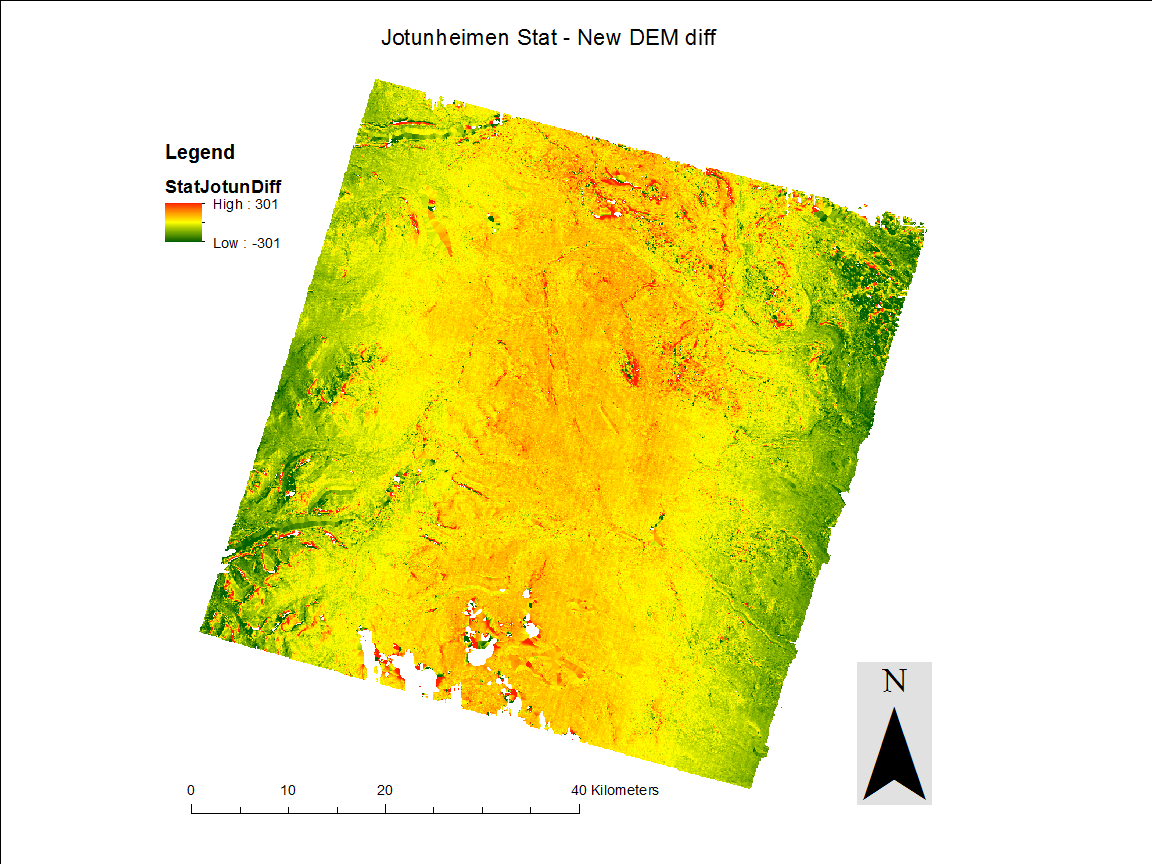
\includegraphics[height=5cm]{StatJotunDiff}
		  \caption{Stat DEM - New DEM}
		  \label{SJD}
	\end{subfigure}%
	\begin{subfigure}{.5\textwidth}
		  \centering
		  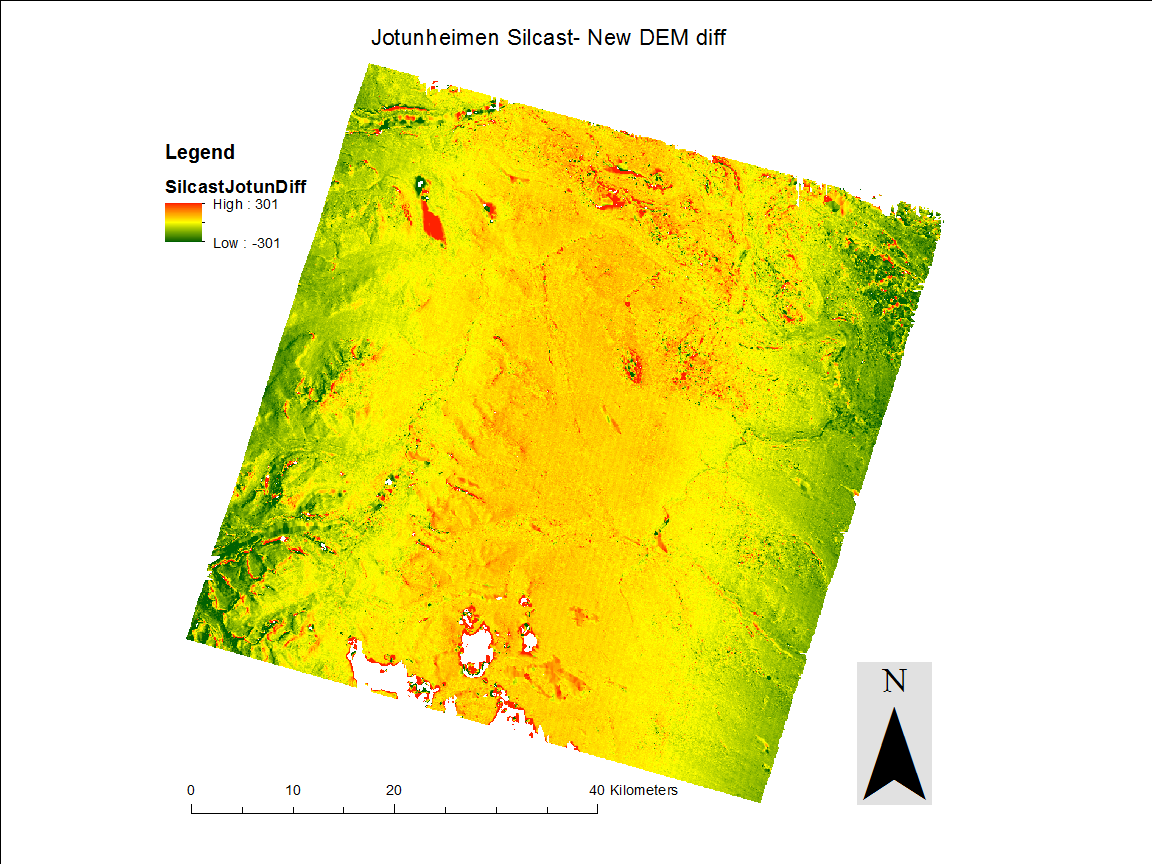
\includegraphics[height=5cm]{SilcastJotunDiff}
		  \caption{SilcAst DEM - New DEM}
		  \label{SiJD}
	\end{subfigure}
	\begin{subfigure}{.5\textwidth}
	 	\centering
	 	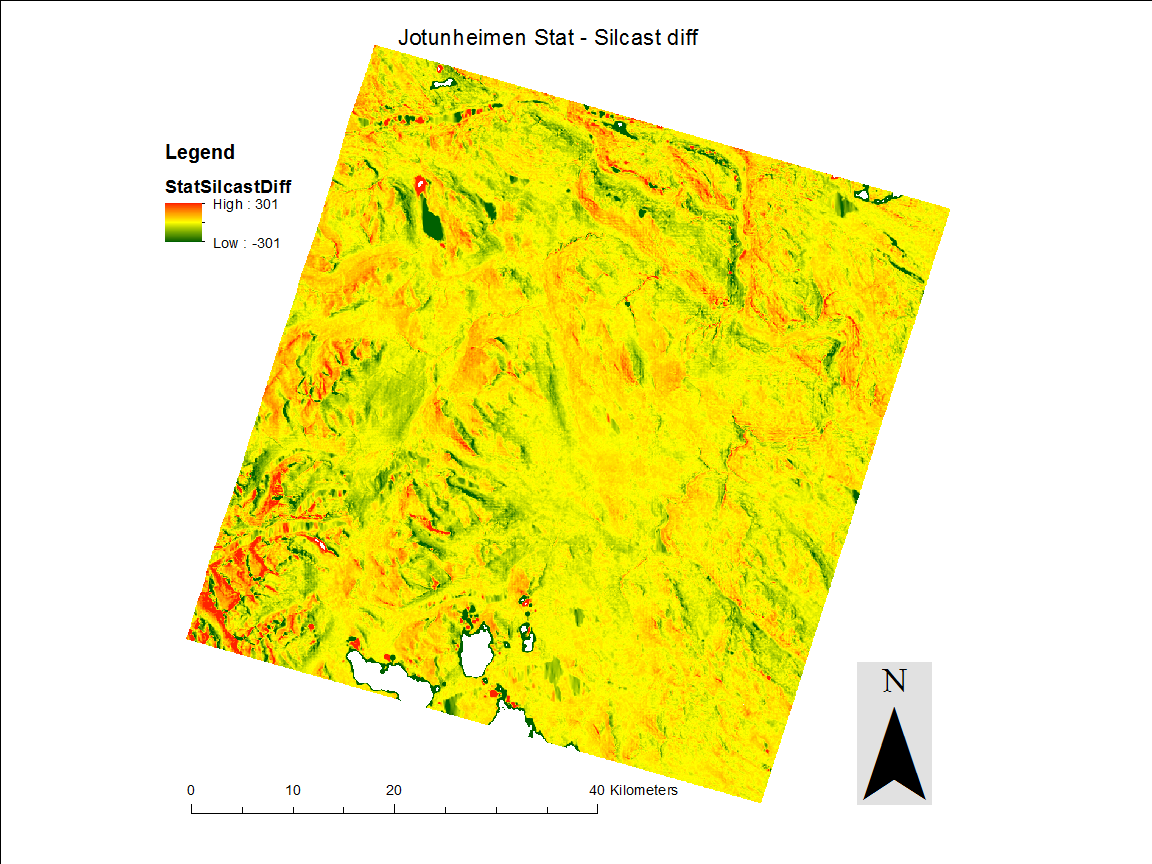
\includegraphics[height=5cm]{StatSilcastDiff}
	 	\caption{StatKart DEM - SilcAst DEM}
	 	\label{SSiD}
	\end{subfigure}
	\caption{The differences of all DEMs}
	\label{diffs}
\end{figure}

\begin{figure}
	\begin{subfigure}{.5\textwidth}
		  \centering
		  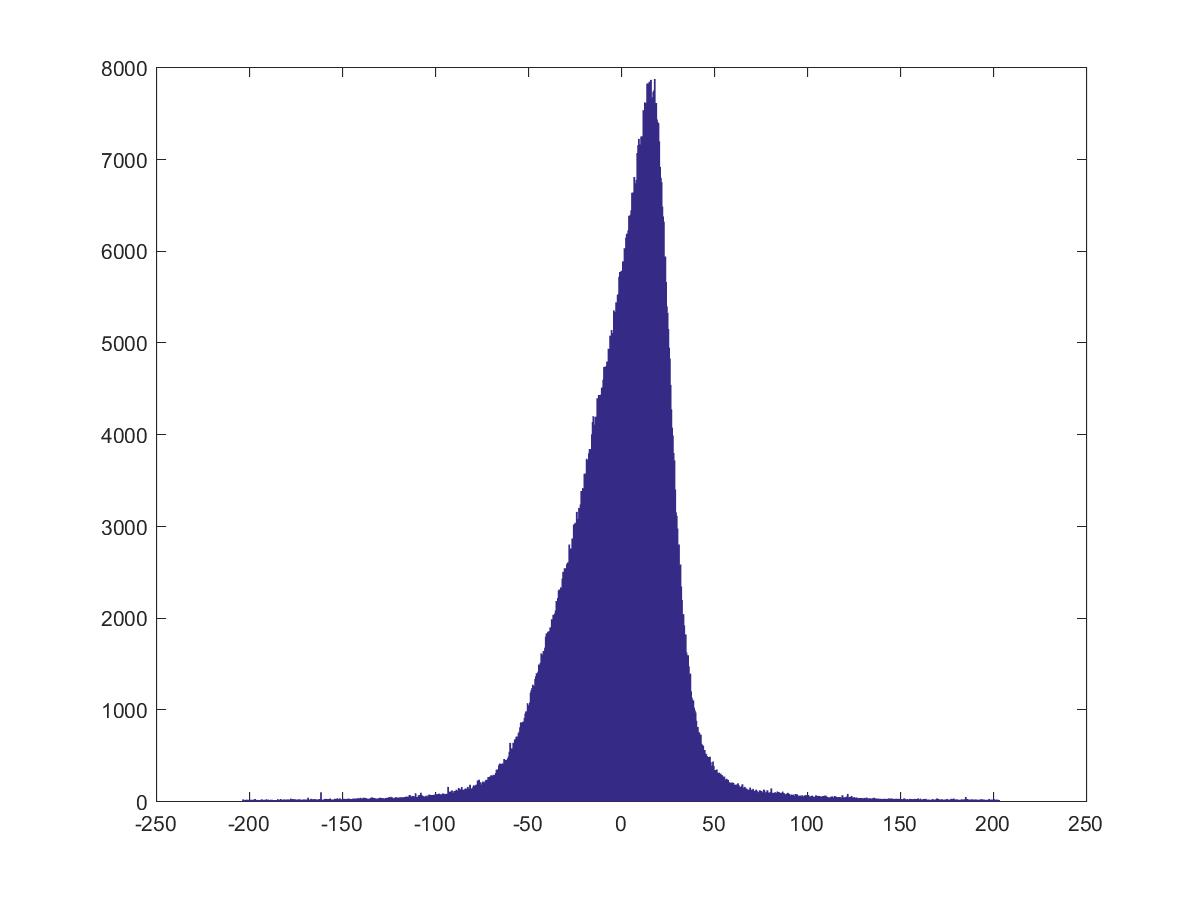
\includegraphics[height=5cm]{hist_SJD}
		  \caption{New DEM - StatKart DEM}
		  \label{histSJD}
	\end{subfigure}%
	\begin{subfigure}{.5\textwidth}
		  \centering
		  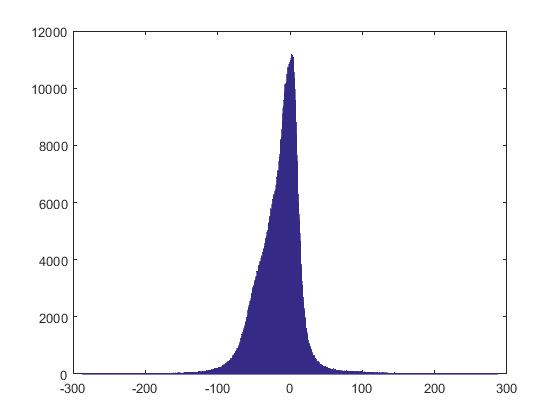
\includegraphics[height=5cm]{hist_SiJD}
		  \caption{New DEM - SilcAst DEM}
		  \label{histSiJD}
	\end{subfigure}
	\begin{subfigure}{.5\textwidth}
	  \centering
	  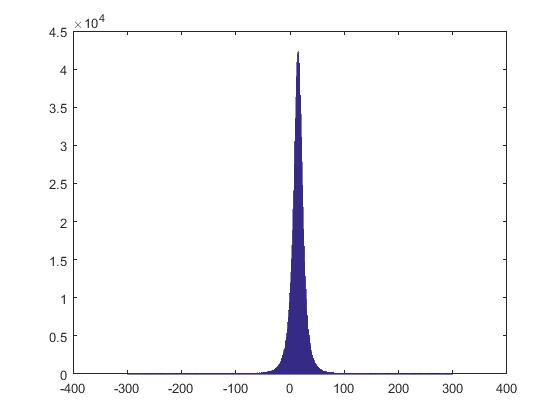
\includegraphics[height=5cm]{hist_SSiD}
	  \caption{StatKart DEM - SilcAst DEM}
	  \label{histSSiD}
	\end{subfigure}
		\caption{A histogram of the values in the all the DEM differances of Jotunheimen}
		\label{hist}
\end{figure}

In figure \ref{hist}, a histogram is presented for all the difference DEM. The histogram for the difference between the statkart and silcast DEM show a histogram that resembles a normal distribution (figure \ref{histSSiD}), while the histogram of the differences between the new DEM and the two others resembles a normal distribution with a left skew (figure \ref{histSJD} and \ref{histSiJD}) . In figure \ref{SJD} and \ref{SiJD}, the green at the borders are quite clear, the center however are more orange then red. This show that the new DEM have been more lifted in the at the boarders, than it have sunken in the center. Witch could explain the left skew in the histogram.


\section{Conclution}

There are definitely biases in the DEM generated from ASTER stereo image in PCI geomatica. The convex bias is likely to occur during the extraction of parallaxes. The reason the parallax isn't extracted properly might have something to do withe the GCPs.

\bibliographystyle{apalike}
\bibliography{kilder}

\end{document}
